\section{Конструкторский раздел}

\subsection{Метод распознавания суицидальных паттернов поведения человека по текстовым сообщениям}

Метод распознавания суицидальных паттернов поведения человека по текстовым сообщениям включает в себя xранение и анализ сообщений пользователей -- для определения, является ли сообщение суицидальным, используется модель машинного обучения. В качестве обучающей выборки используется дополненный датасет размеченных сообщений из открытого доступа \cite{dataset}.

\subsection{Формат и метод сбора данных }

В качестве задействованных в анализе данных используются текстовые сообщения и их даты написания, так как представленная зависимость количества смертей от суицида в зависимости от года и месяца говорит о возможной корреляции месяца написания сообщения и его возможной интерпретации.

Для сбора данных задействовано автоматизированное средство сбора суицидальных сообщений в мессенджере Telegram. Интерфейс программного обеспечения позволяет направить в систему хранения два типа сообщений: суицидальные и на суицидальную тематику.

Средство сбора должно предоставлять пользователю следующий функционал:

\begin{enumerate}
\item[1.] Получение информации о проекте;
\item[2.] Получение информации об отличиях суицидальных сообщений и сообщений на суицидальную тематику;
\item[3.] Направление примеров суицидальных сообщений;
\item[4.] Направление примеров сообщений на суицидальную тематику.
\end{enumerate}

Согласно 152-ФЗ ``О персональных данных'', ``персональные данные -- любая информация, относящаяся к прямо или косвенно определенному или определяемому физическому лицу (субъекту персональных данных)'' \cite{fzpers}. Таким образом, к персональным данным можно отнести фамилию, имя и отчество, дату и место рождения, адрес проживания, семейное, социальное и имущественное положение, образование, профессию, доходы и другое. В связи с этим средство сбора информации, не обрабатывает и не хранит никаких персональных данных о пользователях, направивших сообщения.

\subsection{Средства реализации ботов в мессенджере Telegram}

В качестве представленных к использованию в качестве средства реализации бота в мессенджере телеграм могут быть задействованы популярные библиотеки:

\begin{itemize}
	\item Python Telegram Bot \cite{pythonTelegram},
	\item Telebot \cite{telebot},
	\item Node Telegram Bot API \cite{nodeTelegram},
	\item Telegram Bot Kotlin \cite{kotlinTelegram}.
\end{itemize}

Python Telegram Bot -- это библиотека, предоставляющая асинхронный интерфейс на ЯП Python для Telegram Bot API, которая совместима с версиями Python3.8 \cite{Python} и выше. Данная библиотека предоставляет высокий уровень абстракции и позволяет использовать объектно-ориентированный подход. Помимо реализации API, она также содержит ряд классов высокого уровня, упрощающих разработку ботов. Кроме того, проект поддерживает строенную с асинхронным вводом-выводом. \cite{pythonTelegram}

Telebot -- библиотека на Python, содержащая в себе асинхронную и синхронную реализацию Telegram Bot API. Данный проект предоставляет более гибкий и низкоуровневый доступ к API Telegram, чем упомянутый Python Telegram Bot. \cite{telebot}

Node Telegram Bot API -- это библиотека для создания Telegram-ботов с использованием языка JavaScript \cite{js} и платформы NodeJS \cite{nodejs}. Несмотря на распространенное использование, используемая версия API Telegram является устаревшей. \cite{nodeTelegram}

Telegram Bot Kotlin -- это библиотека для создания Telegram-ботов на ЯП Kotlin \cite{Kotlin}. Отличительной особенностью является возможность разработки ботов на платформе Java Virtual Machine \cite{jvm}, а также поддержка Kotlin Coroutines. \cite{kotlinTelegram}

\subsection{Декомпозиция системы}

На рисунке \ref{img:useCase} представлена диаграмма вариантов использования системы.

\begin{figure}[H]
	\centering
	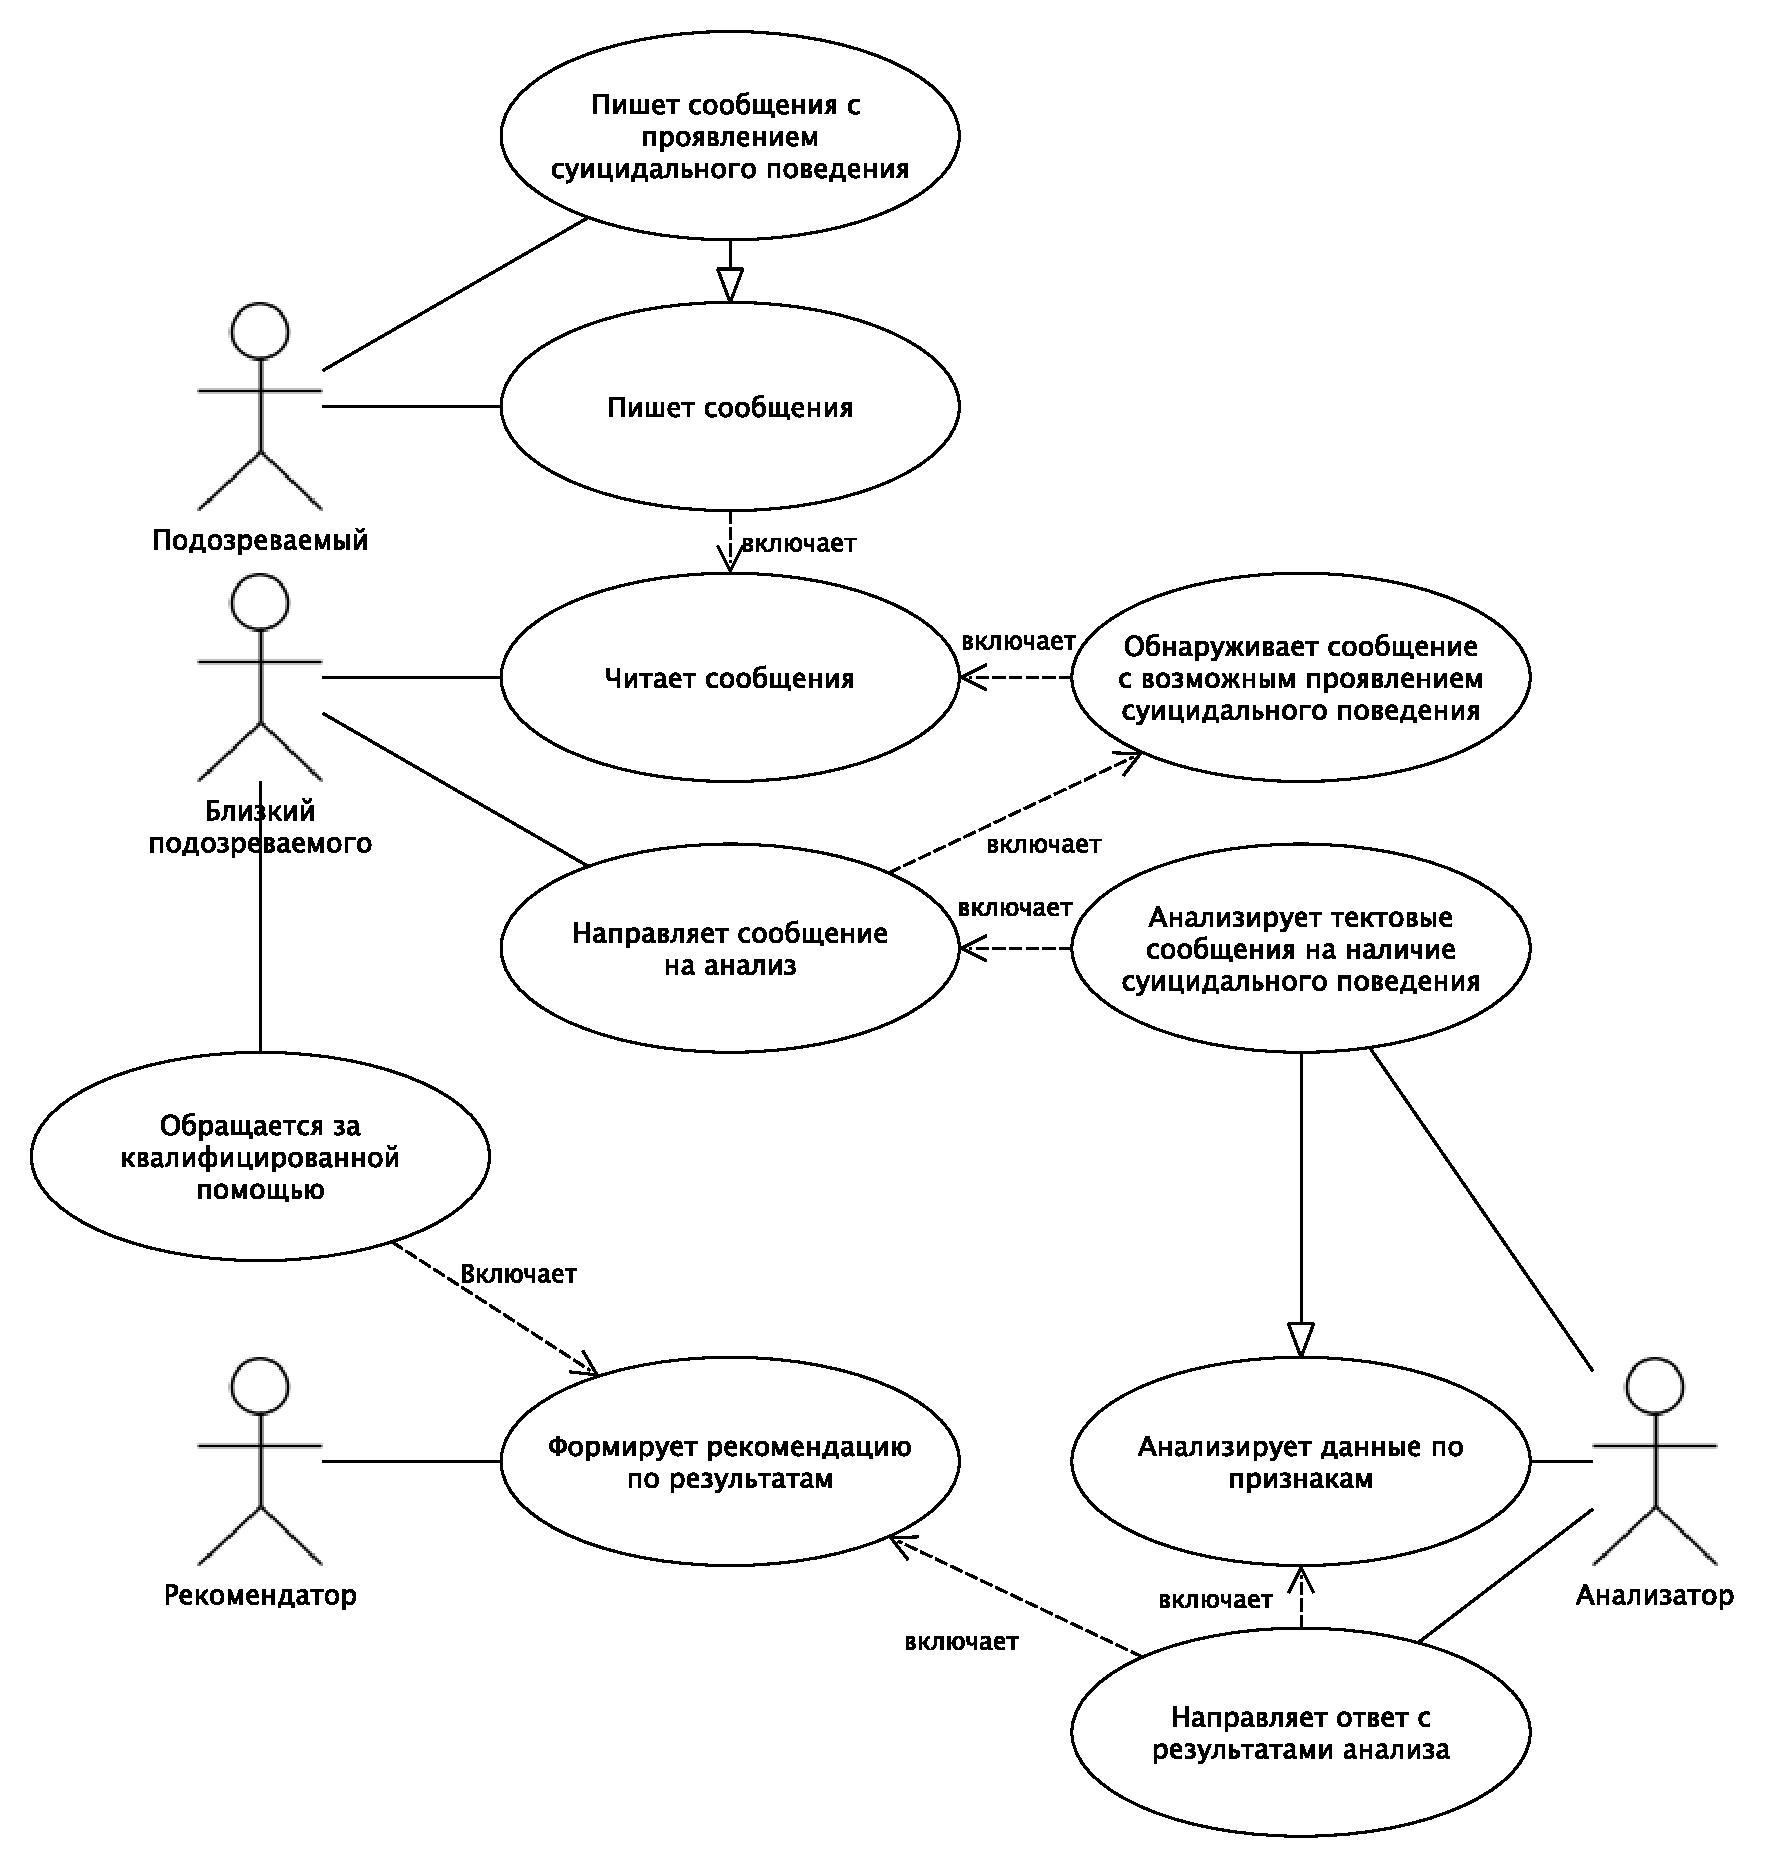
\includegraphics[width=\textwidth]{inc/useCase.pdf}
	\caption{ Диаграмма вариантов использования системы. }
	\label{img:useCase}
\end{figure}

На рисунках \ref{img:idef0}--\ref{img:idef1} представлены IDEF0 диаграммы задачи определения наличия суицидальных паттернов в текстовом сообщении.

\begin{figure}[H]
	\centering
	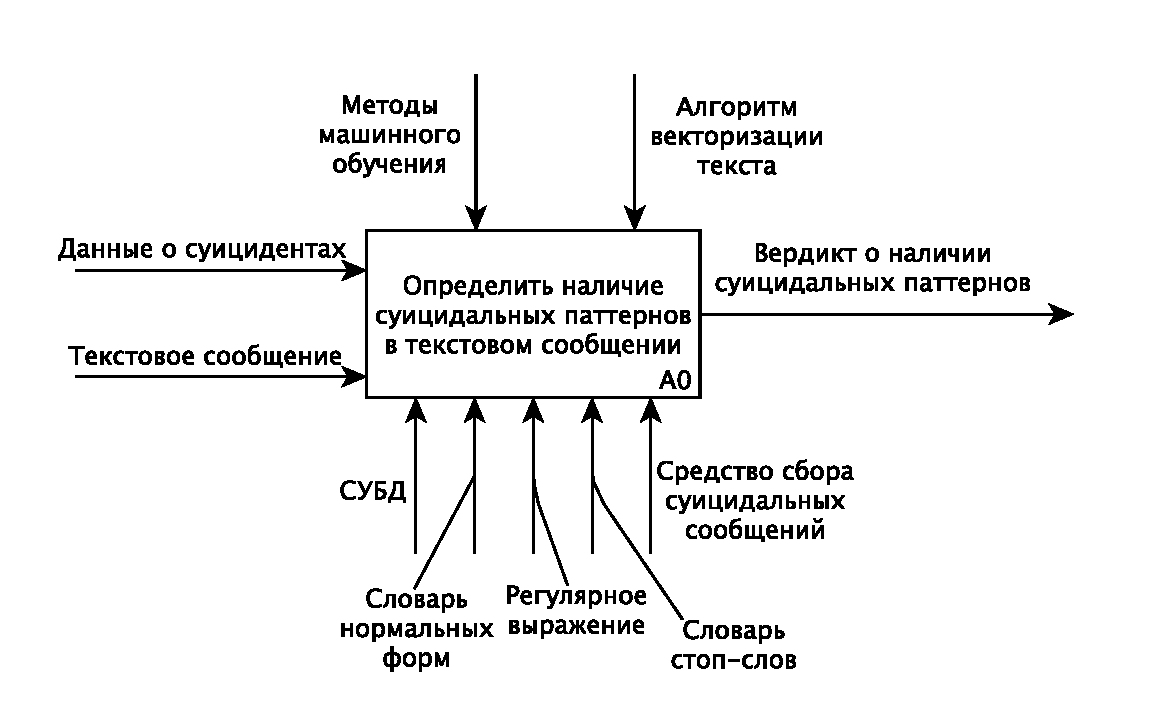
\includegraphics[width=\textwidth]{inc/A0.pdf}
	\caption{ IDEF0 диаграмма уровня А0. }
	\label{img:idef0}
\end{figure}

\begin{figure}[H]
	\centering
	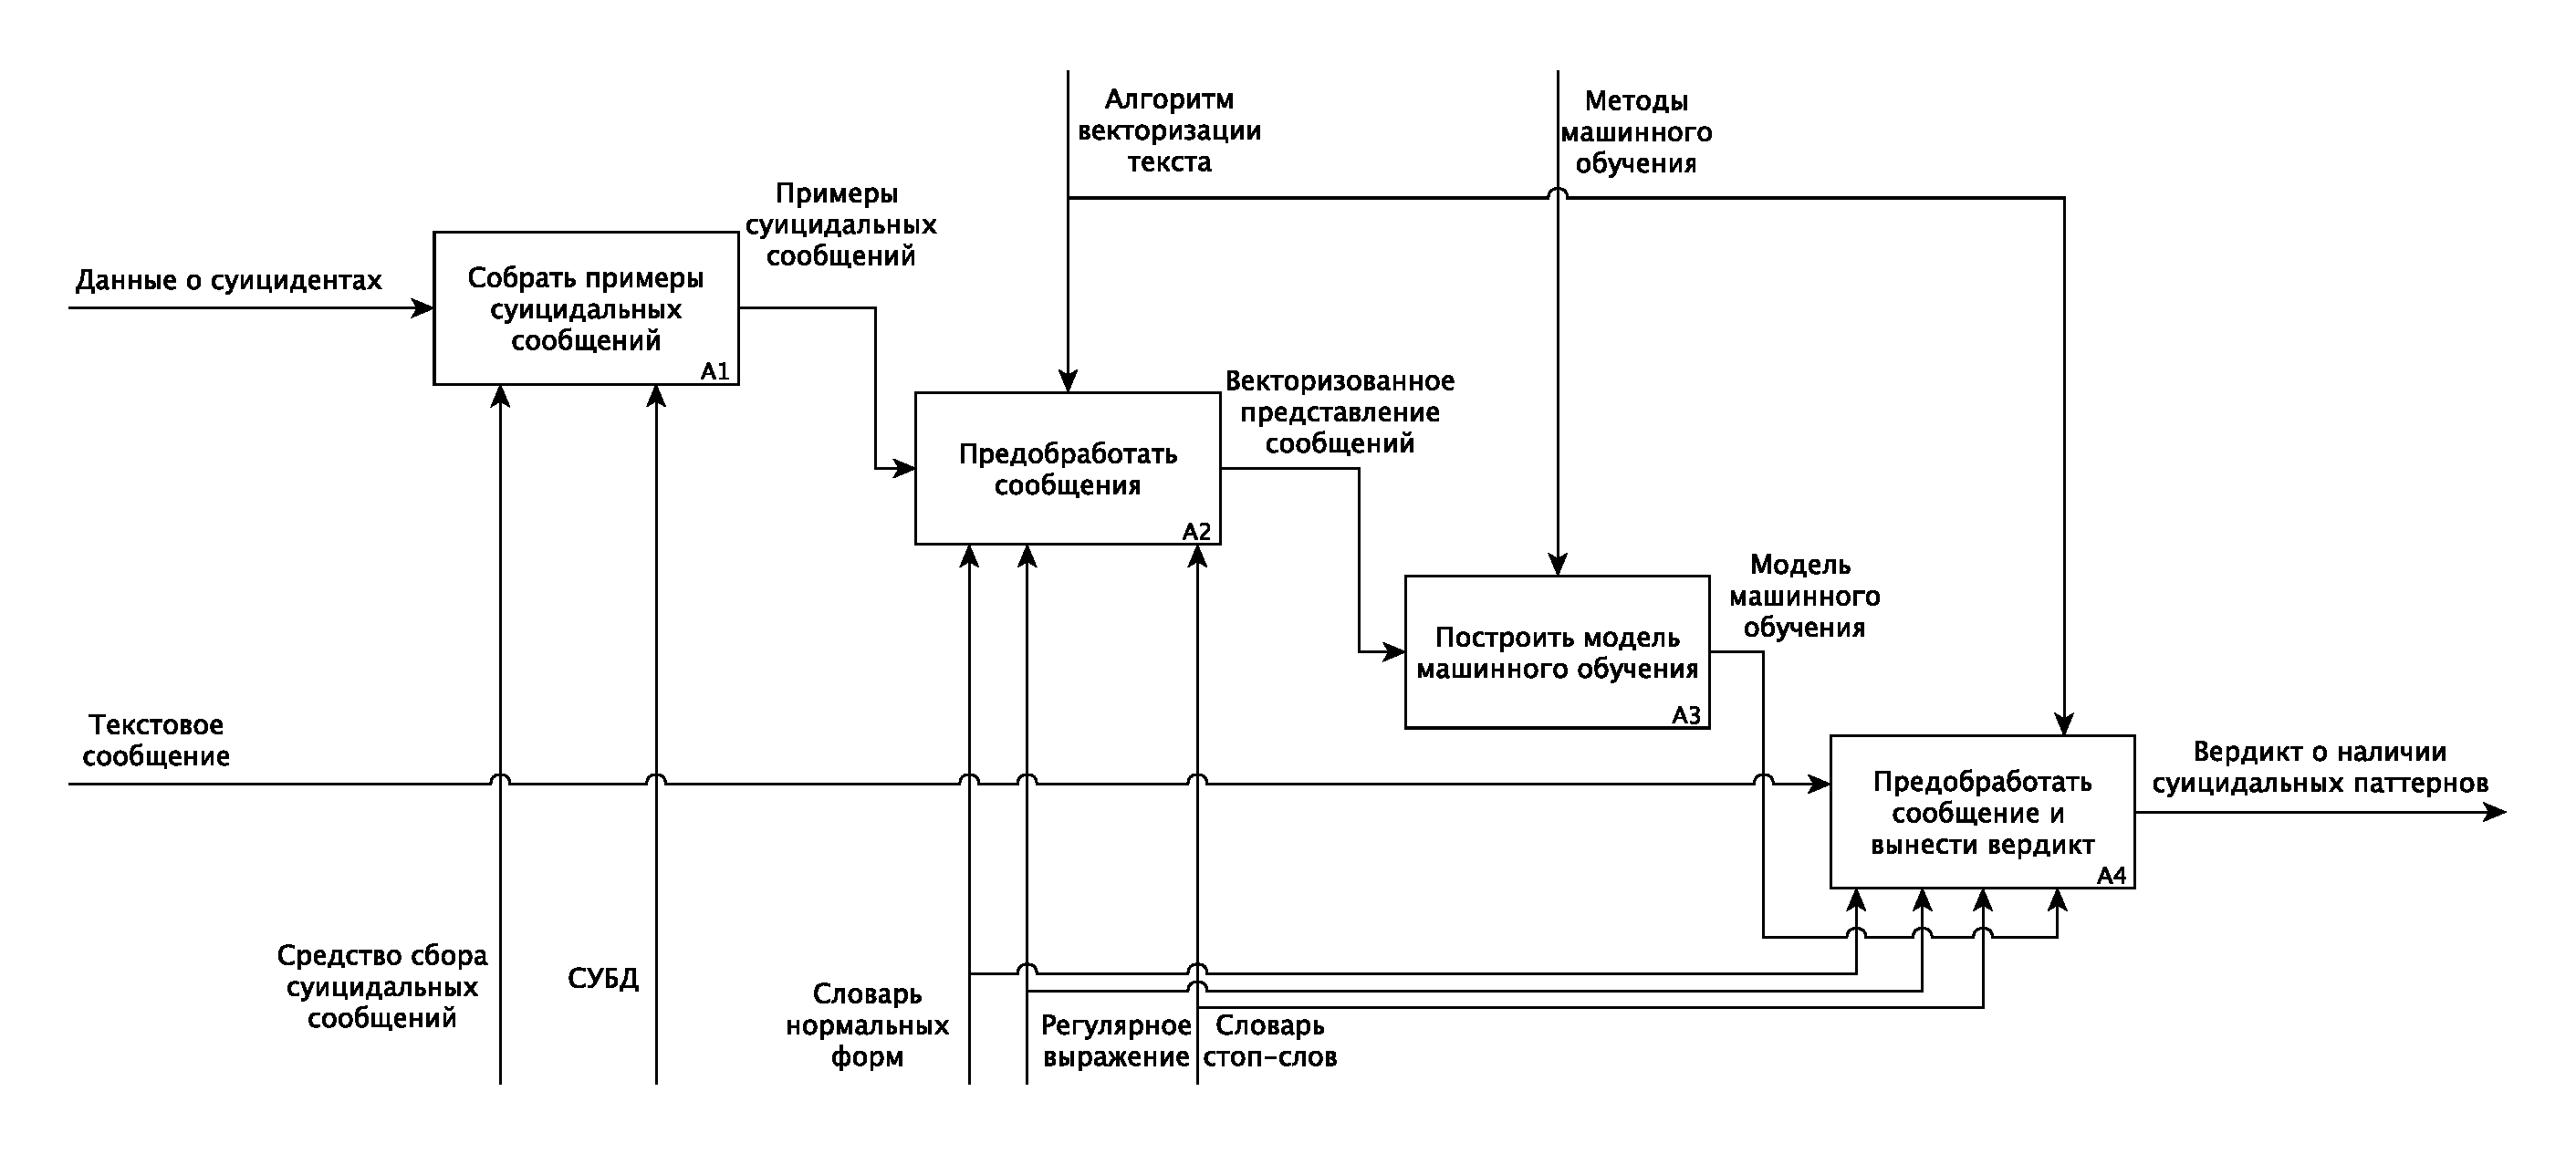
\includegraphics[width=\textwidth]{inc/A1.pdf}
	\caption{ IDEF0 диаграмма уровня А1-A3. }
	\label{img:idef1}
\end{figure}

На рисунке \ref{img:er} представлена диаграмма ``сущность-связь'' в нотации Чена.

\begin{figure}[H]
	\centering
	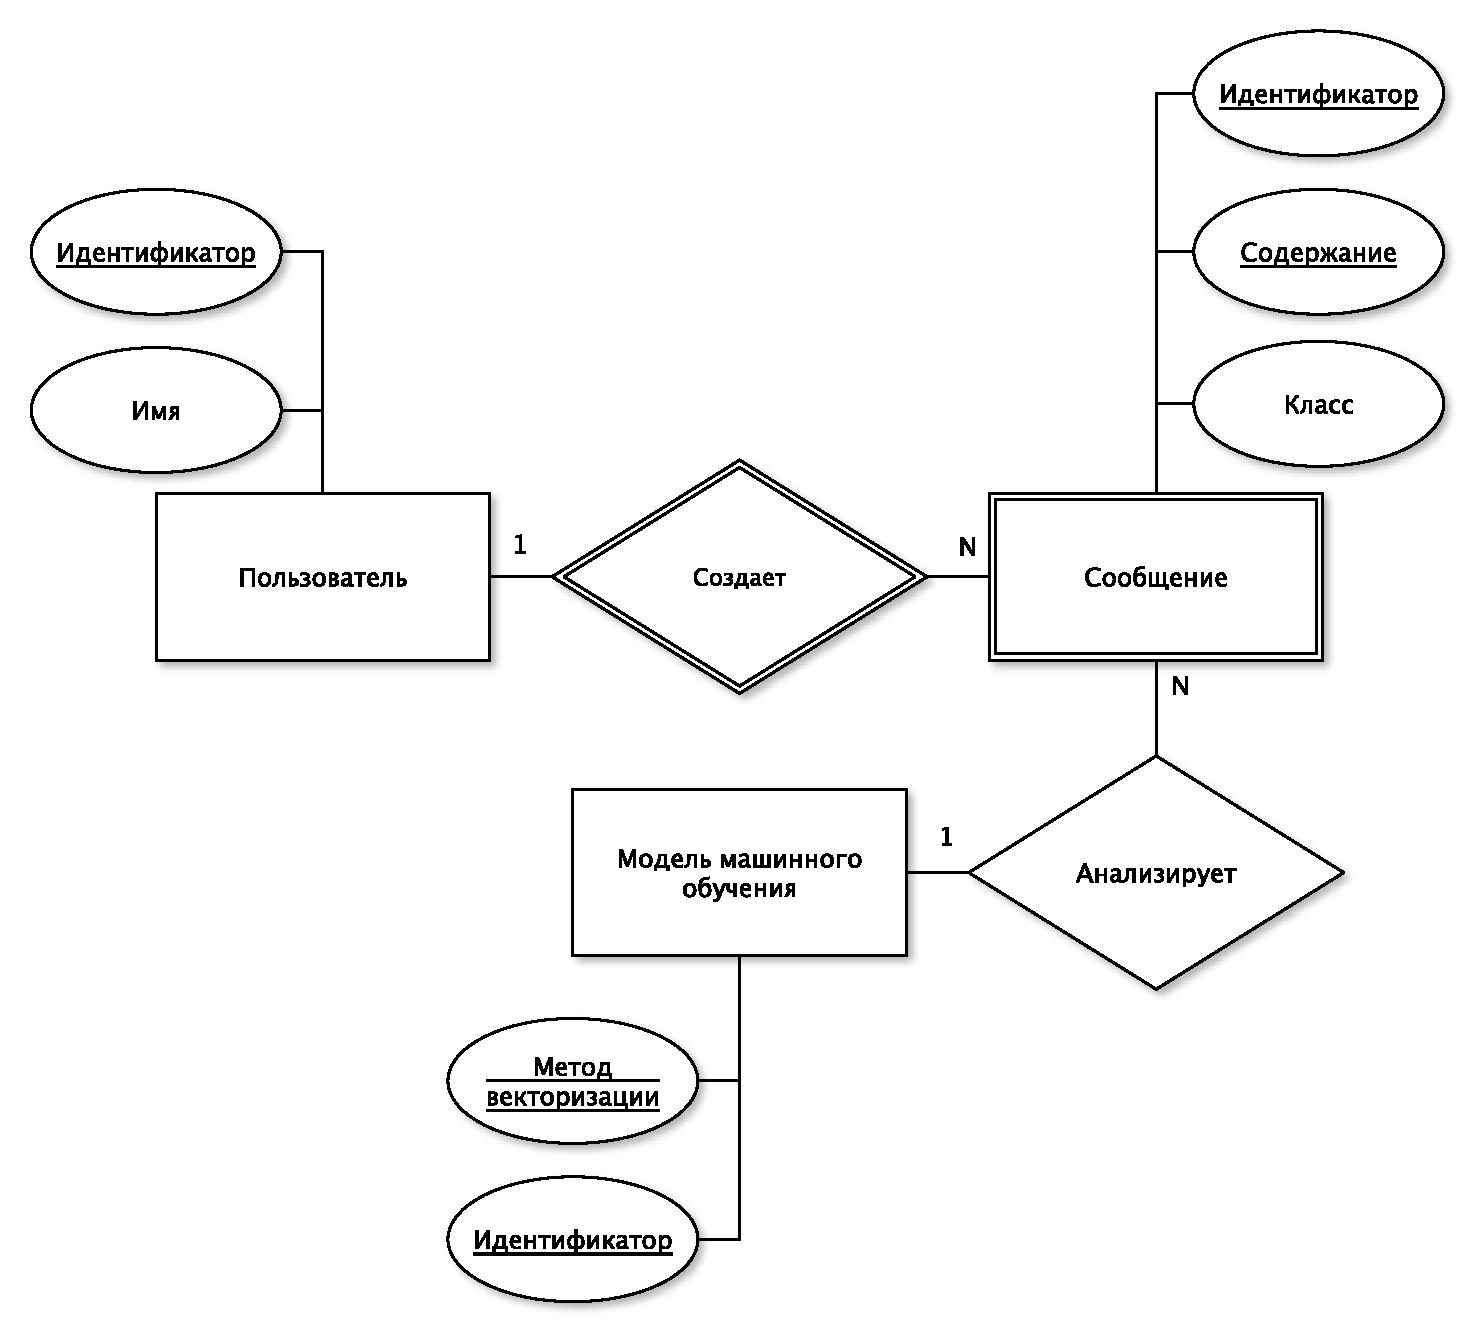
\includegraphics[width=\textwidth]{inc/er.pdf}
	\caption{ Диаграмма ``сущность-связь'' в нотации Чена. }
	\label{img:er}
\end{figure}

\subsection{Задействованные методы машинного обучения}

В качестве задействованных в методе алгоритмов будут рассмотрены: градиентный бустинг, метод случайного леса, метод опорных векторов, метод К-ближайших соседей, логистическая регрессия и перцептрон. Данный список обусловлен потребностью в целях исследования охватить широкий спектр методов машинного обучения для дальнейшего изучения возможности и потребности в создании ансамблевых моделей для решения поставленной задачи.

\subsection{Техника векторизации текстовых сообщений}

Для векторизации собранных текстовых сообщений будут задействованы алгоритм ``мешок слов'' и языковая модель BERT \cite{bert}. Алгоритм TF-IDF не входит в рассмотрение в силу того, что он является модернизацией алгоритма ``мешок слов''. Модели Word2Vec \cite{word2vec} и GloVe \cite{glove} также не попадают в рассмотрение в связи с тем, что данная работа первично имеет цель определить наиболее подходящий для решения задачи алгоритм машинного обучения.

\subsubsection*{Вывод}

wolol

\pagebreak